\documentclass{standalone}
    \usepackage{tikz}
    \usetikzlibrary{circuits.ee.IEC}
    
    \begin{document}
        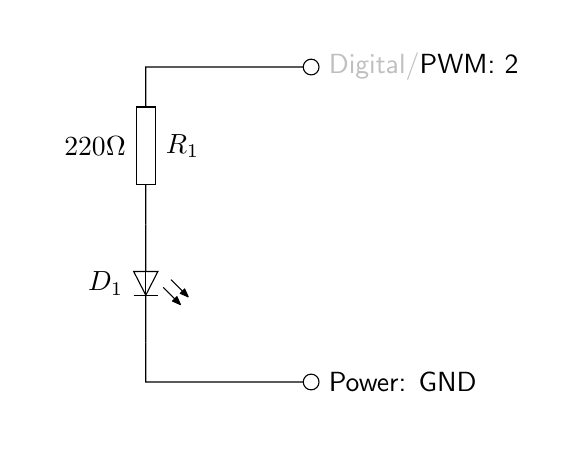
\begin{tikzpicture}[circuit ee IEC]
            % \draw[help lines] grid(10,10);
    
            \draw[draw=none,fill=white] (0.5,0.5) rectangle ++(6.5,5);
    
            \node[anchor=west,font=\sffamily] at (4.2,5) {\textcolor{gray!50}{Digital/}PWM: 2};
            \node[anchor=west,font=\sffamily] at (4.2,1) {Power: GND};
    
            \draw (4.1,5) circle(1mm) ++(-0.1,0) -- ++(-2,0) -- ++(0,-0.5) ++(0,-1) -- ++(0,-0.5) ++(0,-1.5) -- ++(0,-0.5) -- ++(2,0) ++(0.1,0) circle(1mm);
            % \draw (8.1,8) circle (1mm) ++(-0.1,0) -- ++(-5,0) -- ++(0,-1.5) ++(0,-1) -- ++(0,-1.5) ++(0,-3) -- ++(5,0) ++(0.1,0) circle (0.1cm);
            \node at (2,4) [fill=black!20!yellow!60,resistor,ohm=220,rotate=90,fill=none,info'=$R_{1}$] {}; 
            \draw (2,3) to [diode={light emitting,fill=white,info'=$D_{1}$}] ++(0,-1.5); 
        \end{tikzpicture}
    \end{document} 